\section{Global Trigger System overview}\label{sec:fw:gt_system}

The Global Trigger System is based on MicroTCA technology and 10 Gbps optical links. A set of 6 MP7 boards (for MP7 documentation see~\cite{MP7}, for MP7 firmware see~\cite{MP7 firmware}) with a FPGA of the powerful Xilinx Virtex-7 family (XC7VX690TFFG1927-2, see~\cite{Virtex7}) is available. The Global Trigger firmware is implemented on these FPGAs. Every FPGA contains a part of the VHDL representation of a L1 Menu, the partitioning is done by VHDL Producer tool. The trigger decision of every MP7 board is collected on an AMC502 board to generate the "final OR" signal which triggers the readout of the detector.

\begin{figure}[h!]
   \centering
    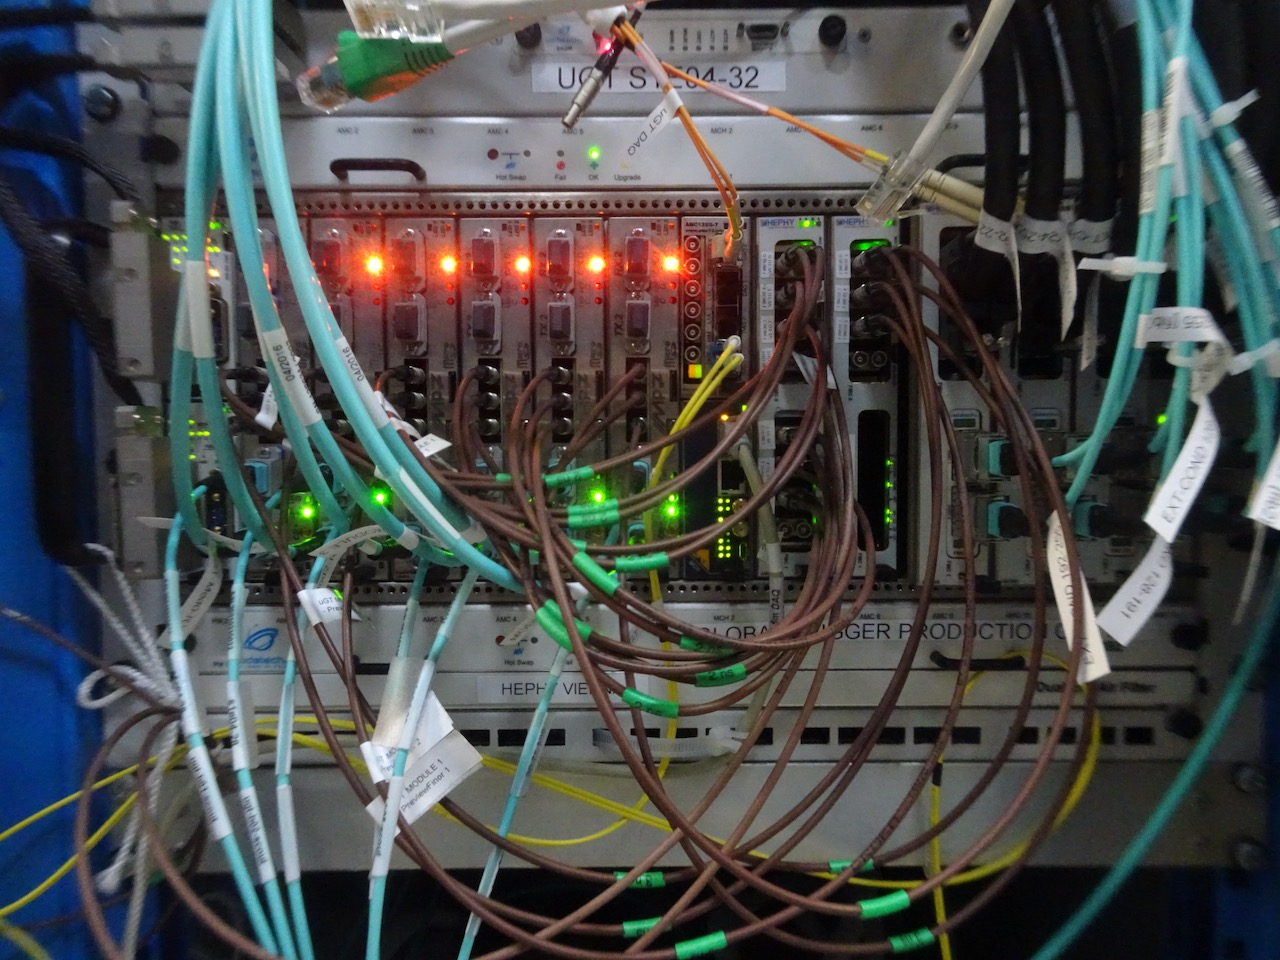
\includegraphics[width=1.0\textwidth]{figures/prodcrate_DSC09437.jpeg}
    \caption{\ugt crate}\label{fig:fw:mgt_crate}
\end{figure}

\section{Firmware overview}\label{sec:fw:fw}
The figure \ref{fig:fw:mgt} shows the architecture of \ugt payload. It consists of framework and the algorithm logic which consists of the following modules:
\begin{enumerate}
\item Global Trigger Logic Data Mapping
\item \ugtl
\item \ufdl
\end{enumerate}

The output mux (part of framework) collects data for read-out record which are send via MP7 read-out to AMC13.

The IPBus system allows the control of hardware via a ‘virtual bus’, using a standard IP-over-gigabit-Ethernet network connection.
\begin{figure}[h!]
   \centering
    \includegraphics[width=1.0\textwidth]{figures/mGT_payload}
    \caption{\ugt payload}\label{fig:fw:mgt}
\end{figure}

\subsection{Firmware versions}\label{sec:fw:fw_version}

This firmware description is based on following versions:
% \begin{itemize}
% \item Framework: \versionframe
% \item Global Trigger Logic: \versiongtl
% \item Final Decision Logic: \versionfdl
% \end{itemize}

\begin{table}[ht]
\caption{Firmware versions}
\vspace{5mm}
\centering
\begin{tabular}{|l|l|}\hline
\textbf{Entity}& \textbf{Version}\\\hline\hline
Global Trigger firmware & \versiongt\\\hline
Framework & \versionframe\\\hline
Global Trigger Logic & \versiongtl\\\hline
Final Decision Logic & \versionfdl\\\hline
\end{tabular}
\label{tab:fw:versions}
\end{table}

\subsection{Directory structure of Global Trigger firmware} \label{sec:fw:dir_struct_gt_fw}

In Global Trigger repository all files for building firmware are in directory \href{\gitbranch/firmware}{\texttt{\textquotesingle firmware\textquotesingle}} with subdirectories for synthesis configuration files (\href{\gitbranch/firmware/cfg}{\texttt{\textquotesingle cfg\textquotesingle }} and \href{\gitbranch/firmware/ucf}{\texttt{\textquotesingle ucf\textquotesingle }}), for VHDL source files (\href{\gitbranch/firmware/hdl}{\texttt{\textquotesingle hdl\textquotesingle }}), for memory files build from IPs (\href{\gitbranch/firmware/ngc}{\texttt{\textquotesingle ngc\textquotesingle }}) and simulation files (\href{\gitbranch/firmware/sim}{\texttt{\textquotesingle sim\textquotesingle }}).\\
All defintions for VHDL code are in \href{\gitbranch/firmware/hdl/packages}{\texttt{\textquotesingle hdl/packages\textquotesingle }}, VHDL source files representing Global Trigger firmware are in \href{\gitbranch/firmware/hdl/payload}{\texttt{\textquotesingle hdl/payload\textquotesingle }} with subdirectories (for \href{\gitbranch/firmware/hdl/payload/gtl}{\texttt{\textquotesingle gtl\textquotesingle }}, \href{\gitbranch/firmware/hdl/payload/fdl}{\texttt{\textquotesingle fdl\textquotesingle }},  \href{\gitbranch/firmware/hdl/payload/frame}{\texttt{\textquotesingle frame\textquotesingle }} and \href{\gitbranch/firmware/hdl/payload/ipbus}{\texttt{\textquotesingle ipbus\textquotesingle }}).

\subsubsection{Implementation in firmware}
\label{sec:fw:implementation_firmware}

Top-of-hierarchy of VHDL code is \href{\gitbranch/firmware/hdl/payload/mp7\_payload.vhd}{\texttt{\textquotesingle mp7\_payload.vhd\textquotesingle }}.

Listing~\ref{lst:fw:mp7_payload_vhd} contains the entity-declaration of the top-of-hierarchy file.

\lstinputlisting[label=lst:fw:mp7_payload_vhd,language=VHDL,caption=Entity declaration of \texttt{mp7\_payload.vhd}]{interfaces/mp7_payload.vhd}

All the declarations for arrays ("type"), parameters ("constant") and look-up-tables ("constant") used in modules are available in \href{\gitbranch/firmware/hdl/packages/gtl\_pkg.vhd}{\texttt{\textquotesingle gtl\_pkg.vhd\textquotesingle }} package-file.

\medskip
\begin{table}
\footnotesize
\caption{Explanation of Listing~\ref{lst:fw:mp7_payload_vhd}}
\vspace{5mm}
\centering
\begin{tabular}{l p{.7\columnwidth}}
\toprule
{Item} & {Explanation}\\
\midrule
\verb|clk| & IPBus clock input.\\
\verb|rst| & IPBus reset input.\\
\verb|ipb_in| & IPBus data input.\\
\verb|ipb_out| & IPBus data output.\\
\verb|clk_payload| & clock inputs [clk\_payload(0)=lhc\_clock].\\
\verb|rst_payload| & reset inputs.\\
\verb|clk_p| & clock 240MHz.\\
\verb|rst_loc| & not used.\\
\verb|clken_loc| & not used.\\
\verb|ctrs| & TTC signals input.\\
\verb|l1a| & L1A signal input.\\
\verb|bc0| & bunch counter reset output.\\
\verb|d| & data input (from optical links).\\
\verb|q| & data output (to optical links).\\
\verb|gpio| & signal outputs to mezzanine board.\\
\verb|gpio_en| & enable (signal) outputs to mezzanine board.\\
\bottomrule
\end{tabular}
\label{tab:gtl:explanation_mp7_payload_vhd}
\end{table}

\clearpage

\subsubsection{Simulation and build of firmware}
\label{sec:fw:sim_build_firmware}

In document \href{\gitbranch/README.md}{\texttt{\textquotesingle README.md\textquotesingle }} one can find instructions for setting up simulation and build environments. For simulation and building of firmware access rights to GitLab (MP7 firmware) are mandatory.

\subsubsection{Testing firmware}
\label{sec:fw:testing_firmware}

Testing of firmware in hardware at CMS P5 (see \ref{sec:app:app_e}) is done with script "multiboard\_function\_test" ("tdf run\ multiboard\_function\_test -h"). Therefore a XML file of the L1Menu and a test vector file must be available at the crate. The firmware of the L1Menu which should be tested must be loaded into the 6 MP7 boards before testing ("tdf run uploadfw\_gt -h"). For checking crate status execute "tdf run crate\_status".\\
This testing is restricted to persons with access to \ugt crates at P5.

\clearpage
